%! TEX program = xelatex
%! TEX root = ../root.tex

\section{实验原理}
\subsection{指令格式}
RV32I的指令格式大致分为一下6种,每种指令都是32位指令,所以指令在内存中必须以4字节对齐。\\

\begin{figure}[H] %H为当前位置,!htb为忽略美学标准,htbp为浮动图形
    \centering %图片居中
    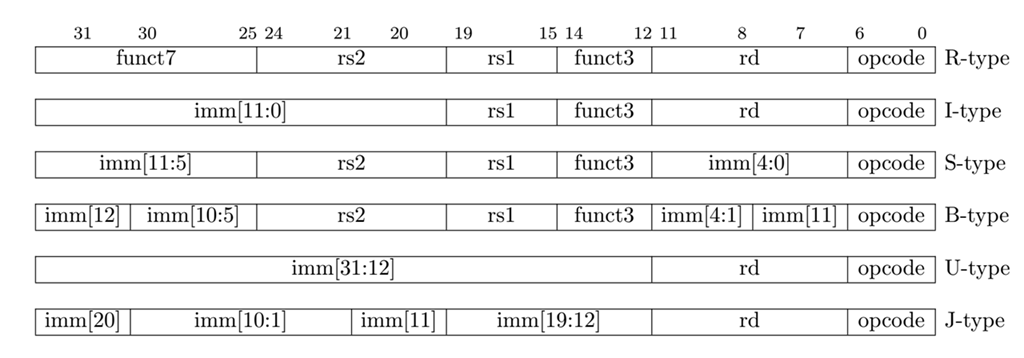
\includegraphics[width=1.0\textwidth]{指令格式.png} %插入图片,[]中设置图片大小,{}中是图片文件名
    \caption{指令格式} %最终文档中希望显示的图片标题
    \label{Fig.1} %用于文内引用的标签
\end{figure}

每种指令格式对应者一类或者多类指令,根据每种指令实现需要的条件,对指令格式也有不同的要求,操作码也各不相同 \\

\begin{tabular}{|l|c|r|}
    \hline
    操作 & 操作码& 包含指令\\
    \hline
    R-type & 0110011 & add, sub, sll, slt, sltu, xor, srl, sra, or, and \\
    \hline
    Arithmetic I-type & 0010011 & addi,  slli, srli, srai, andi, ori, xori, slti, sltui \\
    \hline
    load I-type & 0000011 & lw \\
    \hline
    jump I-type & 1100111 & jalr \\
    \hline
    S-type & 0100011 & sw \\
    \hline 
    B-type & 1100011 & beq, bne, blt, bge, bltu, bgeu \\
    \hline
    U-type(lui) & 0110111 & lui \\
    \hline
    U-type(auipc) & 0010111 & auipc \\
    \hline
    J-type & 1101111 & jal \\
    \hline
\end{tabular} \\

根据指令格式,我们可以从中知道立即数的存储方式:\\

\begin{tabular}{|r|l|}
    \hline
    操作类型 & 立即数组织方式 \\
    \hline 
    I-type & Imm = \{ {21\{Ins[31]}\}, Ins[30:25], Ins[24:21], Ins[20] \} \\
    \hline
    S-type & Imm = \{ \{21\{Ins[31]\}\}, Ins[30:25], Ins[11:8], Ins[7] \} \\
    \hline
    U-type & Imm = \{ Ins[31], Ins[30:20], Ins[19:12], 12'b0 \} \\
    \hline
    J-type & Imm = \{ \{12\{Ins[31]\}\}, Ins[19:12], Ins[20], Ins[30:25], Ins[24:21], 1'b0 \} \\
    \hline
    B-type & Imm = \{ \{20\{Ins[31]\}\}, Ins[7], Ins[30:25], Ins[11:8], 1'b0\} \\
    \hline
\end{tabular} \\

需要注意的是,之所以U-type、J-type、B-type指令的立即数需要末尾加0,与PC地址恒为2的倍数有关,省略恒为0的最末尾可以使得立即数表示大一倍,可能我们会注意到PC地址
实际上恒为4的倍数,为什么不直接省略末尾两个0呢?是因为还有一种2Byte的压缩指令,如果省略两位,那它将无法表示。

\subsection{主要部件设计}
设计CPU首先应该对整体结构有深刻的了解,之后再根据需求设计各组成部件与部件接口。
整个五级流水CPU的数据通路图大致如下:

\begin{figure}[H] %H为当前位置,!htb为忽略美学标准,htbp为浮动图形
    \centering %图片居中
    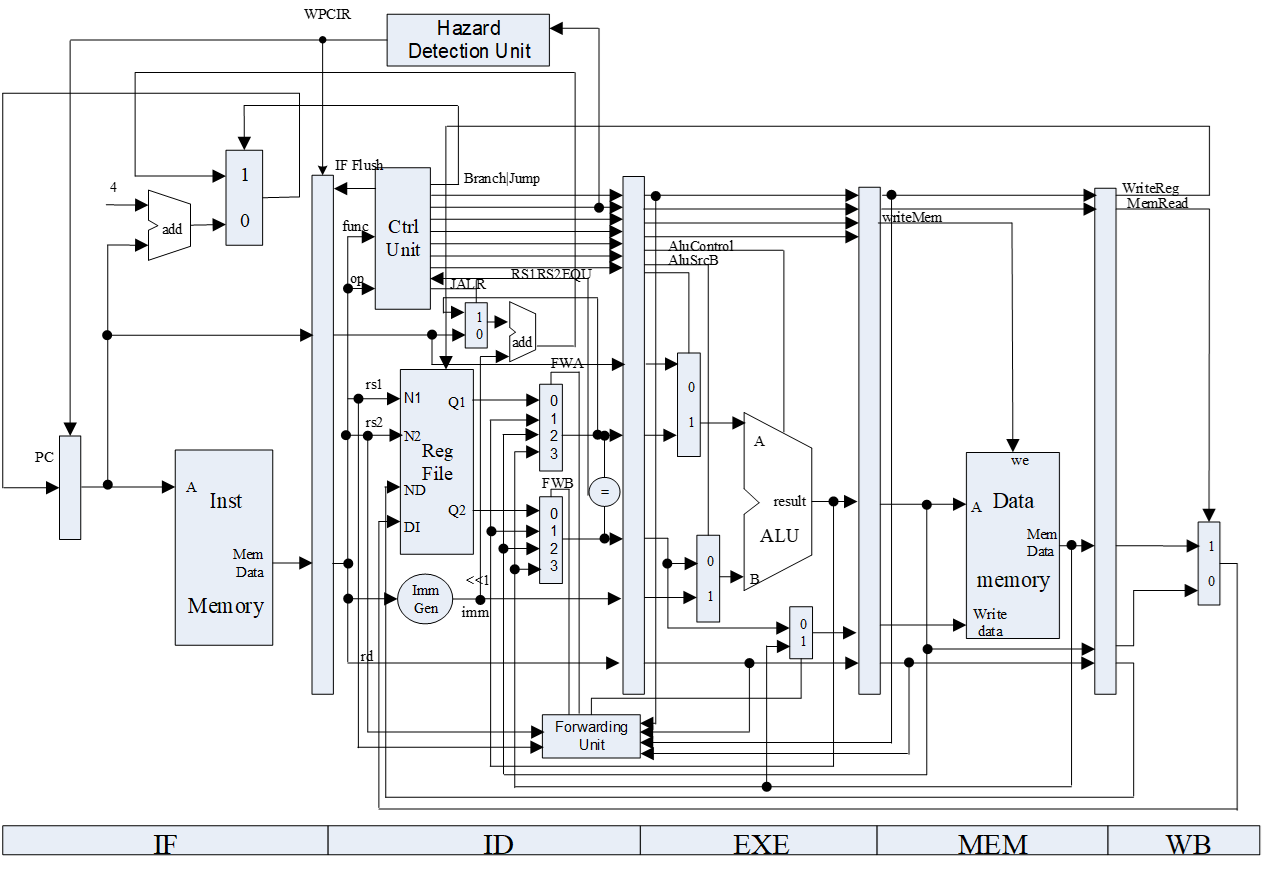
\includegraphics[width=0.7\textwidth]{DataPath.png} %插入图片,[]中设置图片大小,{}中是图片文件名
    \caption{数据通路} %最终文档中希望显示的图片标题
    \label{Fig.2} %用于文内引用的标签
\end{figure}

\subparagraph{Control}
本实验中,ControlUnit复杂产生指令的控制信号、ALU的操作信号与比较器的操作信号
在此部分仅说明需要填充的内容,首先是用于判断跳转指令类型的信号,根据指令类型(OpCode)与funct3判断其类型。

\begin{tabular}{|r|c|c|c|c|l|}
    \hline
    funct3 & 跳转指令类型 & Load类型 & Store类型 \\
    \hline 
    3'b000 & BEQ & LB &  SB \\
    \hline
    3'b001 & BNE & LH & SH \\
    \hline
    3'b010 & - & LW & SW \\
    \hline
    3'b100 & BLT & LBU & - \\
    \hline
    3'b101 & BGE & LHU & - \\
    \hline
    3'b110 & BLTU & - & - \\
    \hline
    3'b111 & BGEU & - & - \\
    \hline
\end{tabular} \\

信号LUI, AUIPC, JAL与JALR只需判断输入OpCode是否等于对应OpCode即可。而Branch跳转控制信号则是JAL, JALR与Branch是否跳转信号(Branch & cmp_res)的或运算,
比较器的控制信号直接将输入的funct3传入即可。
比较重要的是ALU的两个输入口的操作数选择信号,A口选择器有两个输入:PC值(0)与rs1\_data(1),根据指令操作方式我们可以判断出只有AUIPC, JAL与JALR需要在EXE阶段对PC值进行运算,所以它们的控制信号应该置0,其他指令均置1;
B口选择器也有两个输入rs2\_data与立即数,根据指令操作方式我们判断出I类型指令,Load类型指令,Store类型指令,LUI与AUIPC均需要在EXE阶段利用立即数进行计算。 \\
rs1use与rs2use分别是寄存器的rs1与rs2是否被使用的信号,根据前述指令类型我们可以比较容易的得到结果。 \\
最后是hazard_optype信号,此信号用于传递给HazardUnit以便识别当前指令的类型,这个信号的使用可以减少很多信号的传递。

\begin{lstlisting}[language = {verilog}]
module CtrlUnit(
    input[31:0] inst,
    input cmp_res,
    output Branch, ALUSrc_A, ALUSrc_B, DatatoReg, RegWrite, mem_w,
        MIO, rs1use, rs2use,
    output [1:0] hazard_optype,
    output [2:0] ImmSel, cmp_ctrl,
    output [3:0] ALUControl,
    output JALR
);

    //跳转指令的类型判断信号
    wire BEQ = Bop & funct3_0;                    //to fill sth. in 
    wire BNE = Bop & funct3_1;                    //to fill sth. in 
    wire BLT = Bop & funct3_4;                    //to fill sth. in 
    wire BGE = Bop & funct3_5;                    //to fill sth. in 
    wire BLTU = Bop & funct3_6;                   //to fill sth. in 
    wire BGEU = Bop & funct3_7;                   //to fill sth. in 
    //Load指令的类型判断
    wire LB = Lop & funct3_0;                     //to fill sth. in 
    wire LH = Lop & funct3_1;                     //to fill sth. in 
    wire LW = Lop & funct3_2;                     //to fill sth. in 
    wire LBU =Lop & funct3_4;                     //to fill sth. in 
    wire LHU =Lop & funct3_5;                     //to fill sth. in 
    //Store指令的类型判断
    wire SB = Sop & funct3_0;                     //to fill sth. in 
    wire SH = Sop & funct3_1;                     //to fill sth. in 
    wire SW = Sop & funct3_2;                     //to fill sth. in 
    
    wire LUI   = opcode == 7'b0110111;            //to fill sth. in 
    wire AUIPC = opcode == 7'b0010111;            //to fill sth. in 

    wire JAL  = opcode == 7'b1101111;              //to fill sth. in 
    assign JALR = opcode == 7'b1100111;            //to fill sth. in 
    //跳转总控制信号
    assign Branch = (cmp_res & B_valid) | JAL | JALR;   //to fill sth. in 
    //比较器控制信号
    assign cmp_ctrl = funct3;                           //to fill sth. in 
    //ALU的A操作数选择信号
    assign ALUSrc_A = (AUIPC | JAL | JALR) ? 0 : 1;           //to fill sth. in 
    //ALU的B操作数选择信号
    assign ALUSrc_B = (I_valid | L_valid | S_valid | LUI | AUIPC)? 1 : 0;   //to fill sth. in 

    assign rs1use = R_valid|S_valid|B_valid|L_valid|I_valid;         //to fill sth. in 

    assign rs2use = R_valid|S_valid|B_valid;                         //to fill sth. in 

    assign hazard_optype = (R_valid | I_valid | LUI | AUIPC | JAL | JALR) ? 2'b00:
                            S_valid ? 2'b01:
                            L_valid ? 2'b10:2'b11;                  //to fill sth. in 

endmodule
\end{lstlisting}

在我的实验中Control模块分为两个部分,一个部分是接受Instruction的Operation Code输入的Control\_Unit模块,
此模块根据Opcode识别指令类别,并根据指令类别指定各个信号输出,以及ALU需要执行的操作ALUOp。具体阐述将在控制信号部分阐明

\subparagraph{ALUControl}
此模块接受Control模块的ALUOp输出、Funct3、Funct7作为输入,根据它们判断指令类型,再根据指令需求输出需要
ALU执行何等操作的控制信号。下表说明了基本的控制关系:\\

\begin{tabular}{|r|c|c|c|c|l|}
    \hline
    指令类型 & Funct3 & Funct7 & ALUOp & ALU执行操作 \\
    \hline
    lw or sw or jal & *** & * & 00 & 0000(add) \\
    \hline
    branch & *** & * & 01 & 0001(sub) \\
    \hline
    sub & 000 & 1 & 10 & 0001(sub) \\
    \hline
    add & 000 & 0 & 10 & 0000(add) \\
    \hline
    and & 111 & 0 & 10 & 1001(and) \\
    \hline
    or & 110 & 0 & 10 & 1000(or) \\
    \hline
    slt & 010 & 0 & 10 & 0011(slt) \\ 
    \hline
    sll & 001 & 0 & 10 & 0010(sll) \\
    \hline
    sltu & 011 & 0 & 10 & 0100(sltu) \\
    \hline
    xor & 100 & 0 & 10 & 0101(xor) \\
    \hline
    srl & 101 & 0 & 10 & 0110(srl) \\
    \hline
\end{tabular} \\

这里需要注意的是由于Funct7实际只有起作用,所以这里的Funct7特指的是指令的第31位(Funct7的第二高位),
同时由于算术I-type的除了Funct3稍有不同以外,其他操作都与对应的R-type指令基本相同,这里不再赘述。

\subparagraph{Comperator}
在我的实验中,Comperator与ALU是分开的两个部件,Comperator是当指令为Branch时,根据指令的类型判断
是何等比较操作并输出比较结果Zero的部件。

\subsection{数据通路}
完成了个部件的设计,数据通路就是将各个部分连接起来,保证各功能正常实现的关键部分,下面是总体的原理图

\begin{figure}[H] %H为当前位置,!htb为忽略美学标准,htbp为浮动图形
    \centering %图片居中
    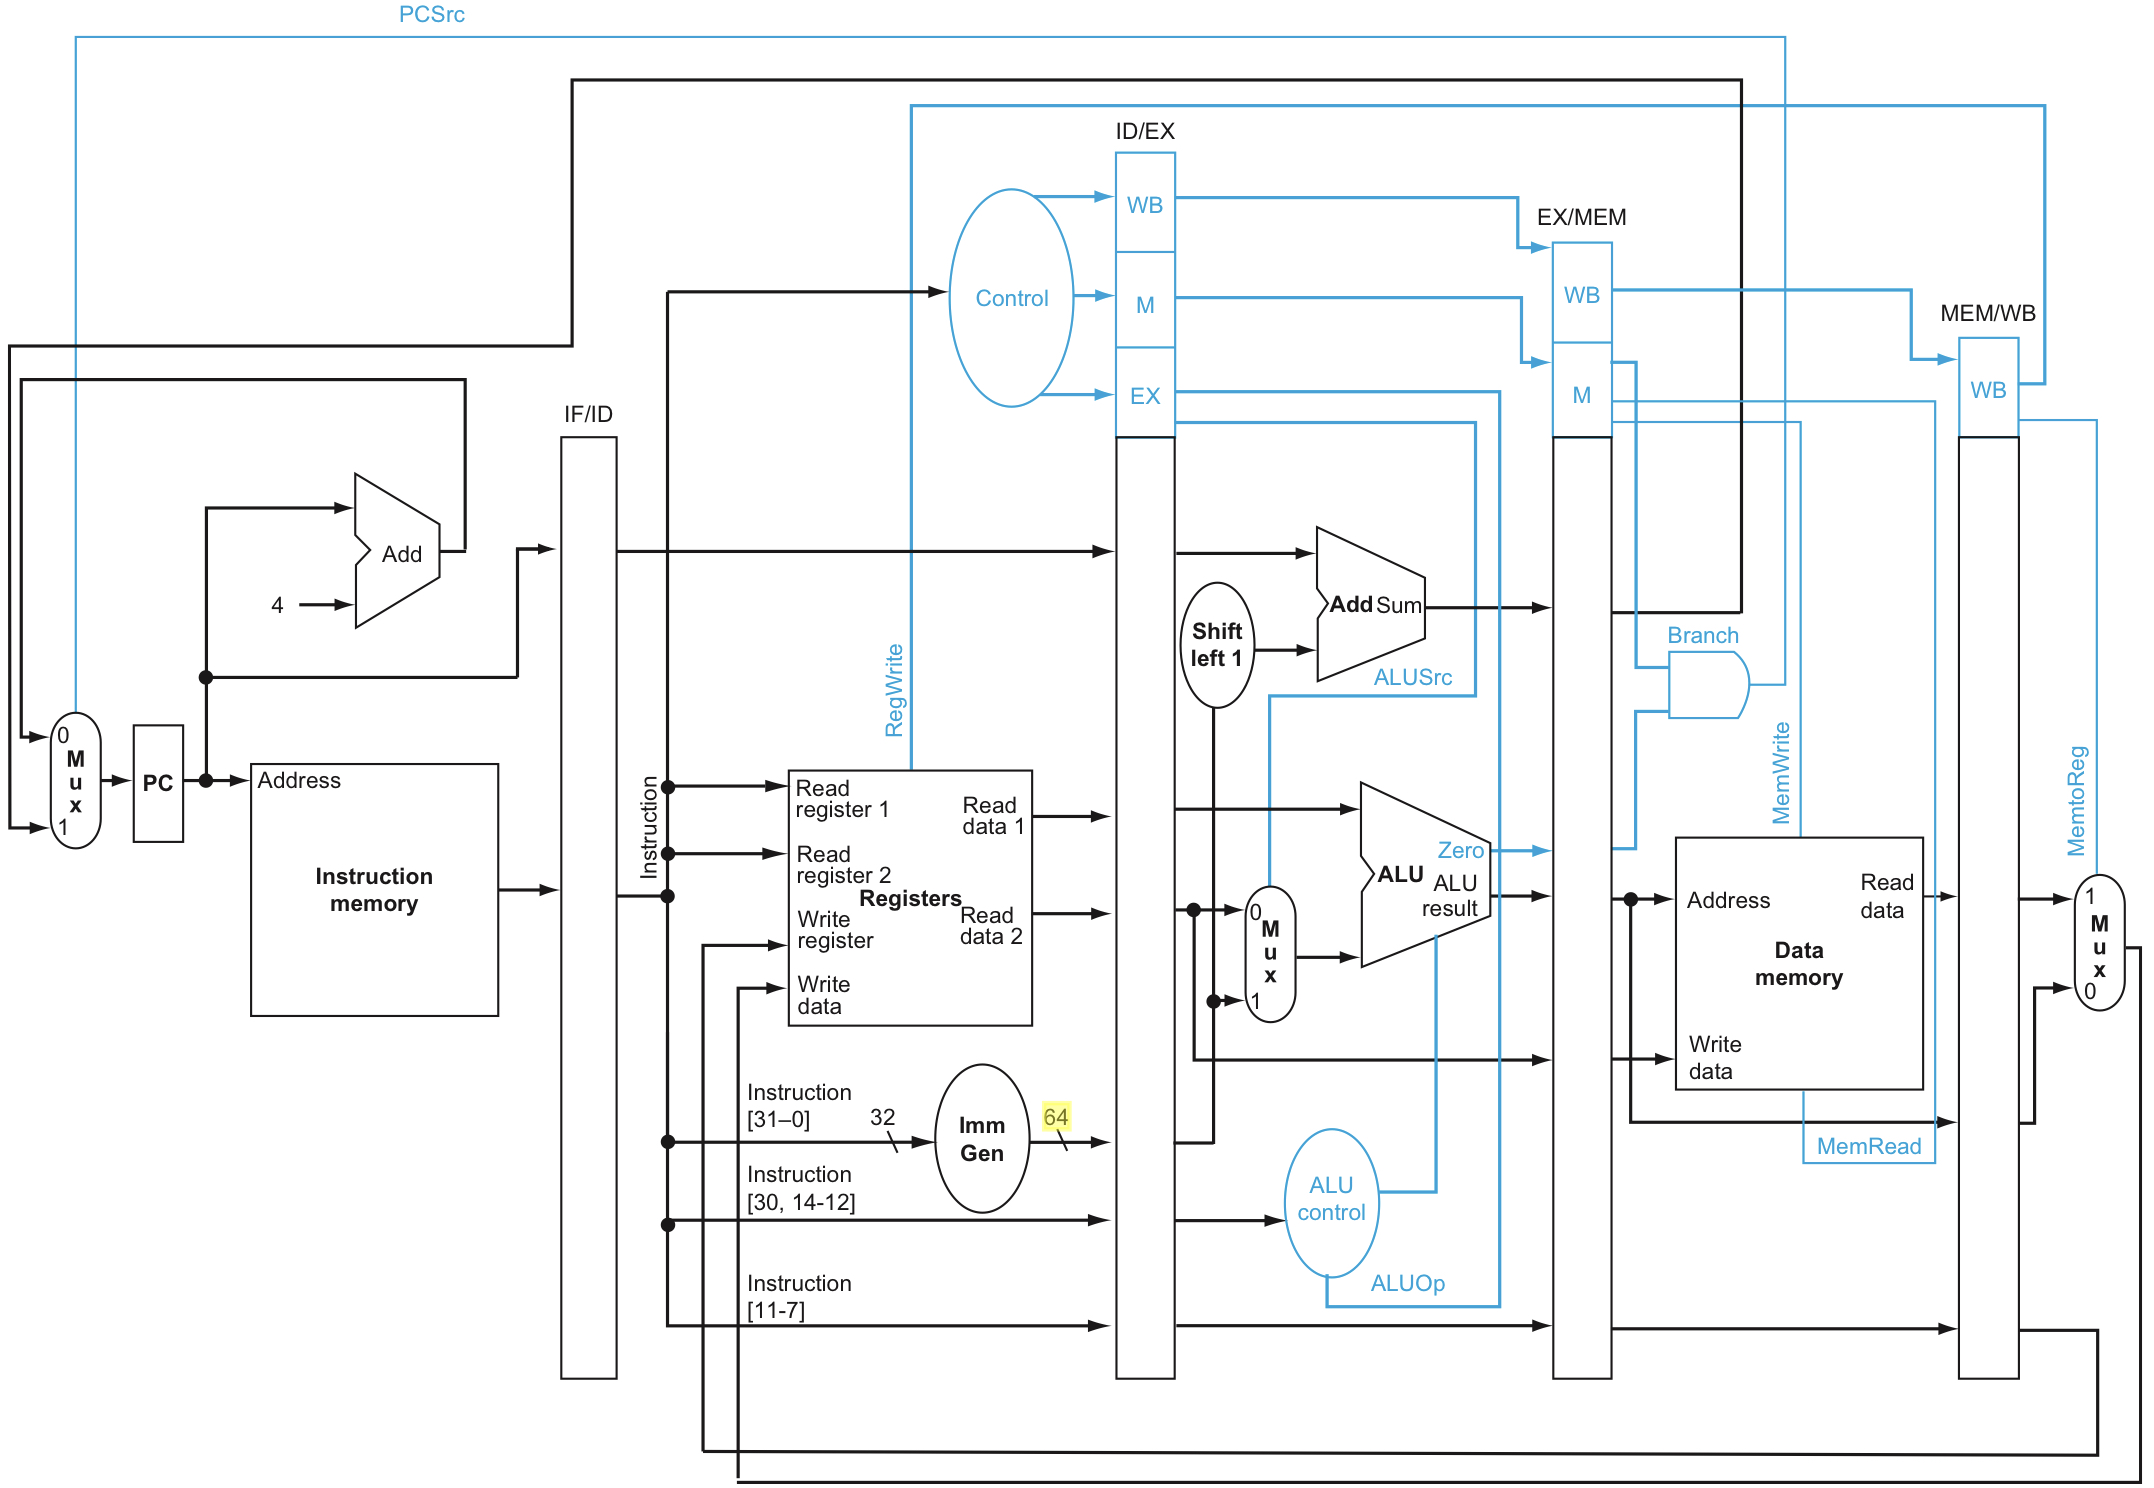
\includegraphics[width=1.0\textwidth]{slide5.jpg} %插入图片,[]中设置图片大小,{}中是图片文件名
    \caption{Datapath} %最终文档中希望显示的图片标题
    \label{Fig.6} %用于文内引用的标签
\end{figure}

\subparagraph{控制信号}
数据通路中最为重要的就是各个控制信号,解释各个控制信号的作用是CPU设计阐述的必要过程 \\

\begin{tabular}{|l|r|}
    \hline
    控制信号 & 控制信号含义 \\
    \hline
    ALUSrc & 决定ALU的操作数之一是来自寄存器的rs2\_val还是立即数 \\
    \hline
    MemtoReg & 决定是否将Data Memory的内容写给寄存器 \\
    \hline
    RegWrite & 决定是否对寄存器进行写入 \\
    \hline
    MemRead & 决定是否用到DMem的数据 \\
    \hline
    BranchANDZero & 决定是否进行Branch跳转 \\
    \hline
    Jump & 决定是否进行Jump跳转 \\
    \hline
    ALUOp & 决定ALU进行何种操作 \\
    \hline
    csr & 决定是否进行csr类操作 \\
    \hline
    lui & 决定是否为lui指令 \\
    \hline
\end{tabular} \\

根据各个指令的操作需求,我们可以得到如下对应关系:\\

\scalebox{0.9}
{
\begin{tabular}{|r|c|c|c|c|c|c|c|l|}
    \hline
    指令类型      & ALUSrc & MemtoReg & RegWrite & MemRead & MemWrite & Branch & Jump & ALUOp \\
    \hline
    R-type       & 0 & 00 & 1 & 0 & 0 & 0 & 0 & 10 \\
    \hline
    LW           & 1 & 01 & 1 & 1 & 0 & 0 & 0 & 00 \\
    \hline
    SW           & 1 & XX & 0 & 0 & 1 & 0 & 0 & 00 \\
    \hline
    B-type       & 0 & XX & 0 & 0 & 0 & 1 & 0 & 01 \\
    \hline
    A I-type     & 1 & 00 & 1 & 0 & 1 & 0 & 0 & 11 \\ %有点问题
    \hline
    UJ-type      & X & 10 & 1 & 0 & 0 & 0 & 1 & XX \\
    \hline  
\end{tabular} 
}

\subsection{latch寄存器}
下面要介绍的是latch寄存器的设计,由于整个流水线被分为IF, ID, EX, MEM, WB五级,所以我们需要四个
段寄存器,并且段寄存器的主要作用是将上一阶段的某些信号值传入下一阶段,并且兼有
置零(Flush)与保持不变(Stall)的作用。

\subparagraph{基本结构} 
段寄存器基本是在时钟上升沿决定相应阶段传入的寄存器值,主要设计结构如下所示:

\begin{lstlisting}[language = {verilog}]
module latch(
    input clk,
    input stall,
    input Flush,
    input A_In,
    input A_Out
);    

    always @(*) begin
        if(~stall) begin
            A_Out <= Flush ? 0 : A_In;
        end
    end
\end{lstlisting}

\subparagraph{信号的传递}
每个阶段之间需要传输的信号是Latch设计中最为重要的部分,由下表给出 \\

\begin{tabular}{|r|l|}
    \hline
    段寄存器 & 信号 \\
    \hline
    IF/ID  & PC, Instruction \\
    \hline
    ID/EX  & All Control Signals, PC, Imm, Instruction \\
    \hline
    EX/MEM & ALUOut, RegWrite, MemWrite, MemtoReg, rd, lui, PC, Imm, Instruction \\
    \hline
    MEM/WB & Mem\_w\_data, RegWrite, MemWrite, MemWrite, PC, Imm, Instruction \\
    \hline
\end{tabular} \\

\subsection{Hazard}
在此次的实验中,Hazard由结构竞争、数据冒险和控制竞争三部分组成,简单起见
本模块被设计在ID阶段,利用段寄存的Flush与Stall功能实现插入bubble或者清空段寄存器数据
并且本次实验还设计了Forward Units以减少停顿次数,提高流水线效率,同时本此实验中实现了Branch No Taken的
跳转策略,在EX阶段识别并执行跳转语句。具体的设计分几部分阐述如下:

\subparagraph{Forword Units}
前送只涉及到EX, MEM, WB三个阶段的数据前送,在此实验中分为ALU的两个数据输入口进行讨论,
其中ALU的1号操作数口接受来自:
1. MEM阶段的上一条指令EX阶段的ALU计算结果
2. WB阶段将要写回Memory的数据结果
3. ID阶段传入的rs1\_val(正常值)
所以前送ALU操作数1口的条件应该是:
\begin{itemize}
    \item [*] EX/MEM.RegisterRd = ID/EX.RegisterRs1
    \item [*] MEM/WB.RegisterRd = ID/EX.RegisterRs1
\end{itemize}
同样的分析可以得到,前送ALU操作数2口的条件应该是:
\begin{itemize}
    \item [*] EX/MEM.RegisterRd = ID/EX.RegisterRs2
    \item [*] MEM/WB.RegisterRd = ID/EX.RegisterRs2
\end{itemize}
这样使得涉及到算数指令的Read After Write冲突无需停顿(插入一个bubble)即可得到正确结果,使得涉及到Load指令的RAW情形仅需一次停顿即可避免数据冲突。

\subparagraph{Branch No Taken}
对于跳转指令的判断,此实验我均是在EX阶段判断并跳转,我采取了Branch No Taken的设计方式:若EX阶段检测到不满足跳转条件(Branch指令不跳转),
则流水线继续执行,若EX阶段检测到跳转(Branch满足跳转条件或Jal, Jalr必定跳转),则将下一条PC地址的值修改为跳转的目标地址,并且将IF/ID, ID/EX段寄存器的值全部
Flush掉(清空),这样可以使得无效指令全部被清空,并且跳转指令的剩下部分继续向后流动直至执行完毕(例如jal, jalr指令还需将PC + 4的值写入寄存器)

\subparagraph{Data Hazard}
由于拥有了前递控制,所以实验中仅需将涉及到Load指令的RAW情形在EX阶段判断并插入bubble,在此实验中,插入bubble的判断条件就变为了:
\begin{itemize}
    \item [*] EX阶段执行的语句是Load指令
    \item [*] WB阶段的RegWrite(寄存器写入使能信号)为高位(要写入寄存器)
    \item [*] EX.RegisterRd = ID.RegisterRs1 或者 EX.RegisterRd = ID.RegisterRs2
\end{itemize}
并且插入bubble的方式就是将EX/MEM段寄存器Flush掉,并使得IF/ID与ID/EX段寄存器Stal(停顿)一个周期